\chapter{GIỚI THIỆU ĐƠN VỊ THỰC TẬP}
\label{chap:gioi_thieu_orlab}

Phòng thí nghiệm Tối ưu hóa các hệ thống lớn (ORLab) trực thuộc Trường Đại học Phenikaa là đơn vị nghiên cứu học thuật chuyên sâu trong hai lĩnh vực mũi nhọn: tối ưu hóa và trí tuệ nhân tạo. Với phương châm kết hợp chặt chẽ giữa lý thuyết toán học giải tích và triển khai kỹ thuật hiệu năng cao, ORLab đóng vai trò tiên phong trong việc phát triển các mô hình tính toán hiện đại để giải quyết các bài toán thực tiễn phức tạp có quy mô dữ liệu lớn.

\section{Thông tin chung về cơ sở thực tập}
\label{sec:thong_tin_chung_orlab}

Các thông tin định danh chính thức của phòng thí nghiệm được công bố trên cổng thông tin khoa học của Lab tại địa chỉ \url{https://www.orlab.vn/} bao gồm:

\begin{itemize}
    \item \textbf{Tên đơn vị}: Phòng thí nghiệm Tối ưu hóa các hệ thống lớn (ORLab).
    \item \textbf{Trưởng phòng thí nghiệm}: PGS.TS. Phạm Văn Cảnh.
    \item \textbf{Cán bộ hướng dẫn nghiên cứu}: TS. Trần Đình Tân.
    \item \textbf{Trụ sở làm việc}: phòng 2211, tầng 22 tòa nhà A9, Trường Đại học Phenikaa, đường Nguyễn Trác, phường Dương Nội, Hà Nội, Việt Nam.
    \item \textbf{Website chính thức}: \url{https://www.orlab.vn/}
\end{itemize}

\begin{figure}[htbp!]
    \centering
    
\includegraphics[width=0.24\textwidth]{Images/orlab/orlab_logo.png}
    \caption[Logo phòng thí nghiệm ORLab]{Logo chính thức của phòng thí nghiệm ORLab.}
    \label{fig:orlab_logo}
\end{figure}

\section{Lịch sử hình thành và sứ mệnh phát triển}
\label{sec:lich_su_orlab}

Được thành lập tại Trường Đại học Phenikaa, ORLab định vị sứ mệnh trở thành trung tâm nghiên cứu xuất sắc về vận trù học, giải thuật tối ưu và ứng dụng trí tuệ nhân tạo. Phòng thí nghiệm tập trung giải quyết các bài toán tối ưu tổ hợp phức tạp thuộc lớp NP-khó xuất hiện trong giao thông vận tải, logistics, chuỗi cung ứng công nghiệp và khoa học sự sống.

Môi trường học thuật tại ORLab đề cao tính chính xác toán học, phương pháp luận thực nghiệm khách quan và khả năng hiện thực hóa thuật toán trên các hệ thống tính toán phân tán và tăng tốc phần cứng. Sinh viên và học viên cao học khi tham gia nghiên cứu tại Lab được rèn luyện quy trình làm việc khoa học chuẩn mực quốc tế: từ khâu phân tích bài toán, xây dựng mô hình giải tích, chứng minh các tính chất cận xấp xỉ, đến khâu thiết kế pipeline thử nghiệm và công bố kết quả.

\section{Cơ cấu tổ chức và nhân sự nghiên cứu}
\label{sec:co_cau_orlab}

Cơ cấu nhân sự của ORLab quy tụ các nhà khoa học giàu kinh nghiệm, các tiến sĩ tốt nghiệp từ các trường đại học uy tín trong và ngoài nước, cùng lực lượng nghiên~cứu~sinh~và~sinh~viên~tài~năng:

\begin{figure}[htbp!]
    \centering
    \begin{minipage}{0.45\textwidth}
        \centering
        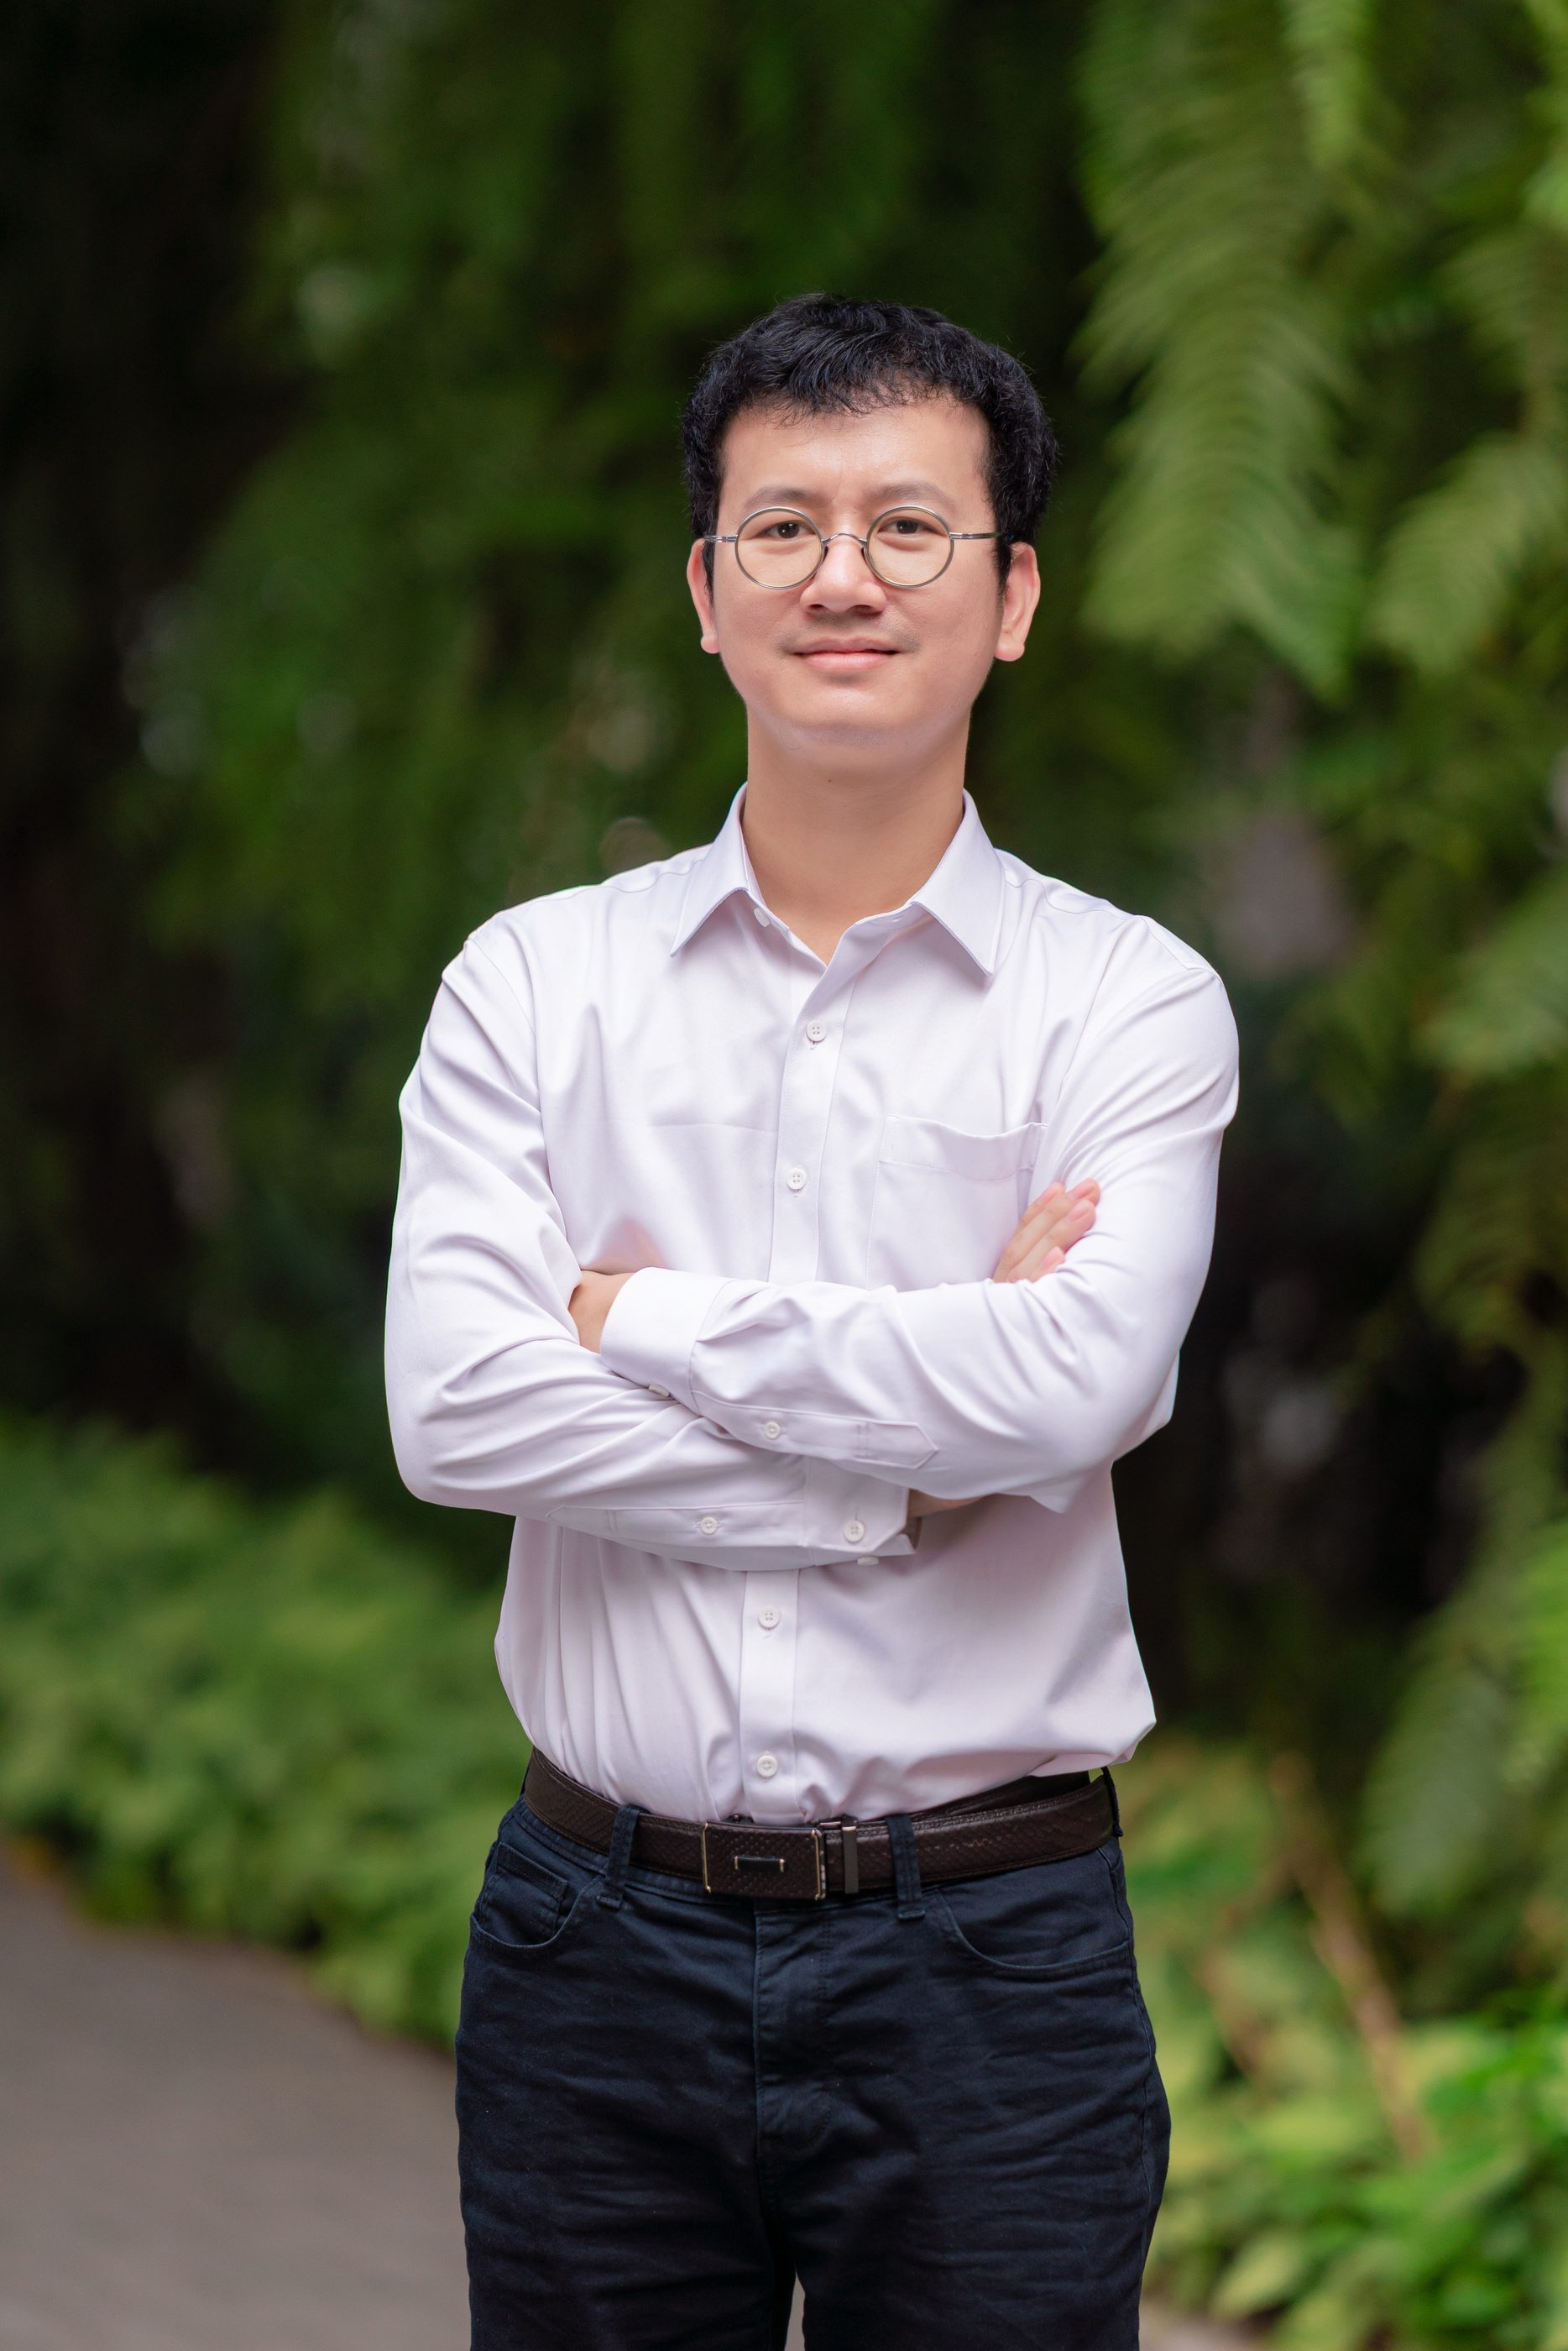
\includegraphics[width=0.34\textwidth,height=4.6cm,keepaspectratio]{Images/orlab/phamvancanh.jpg}\par
        \vspace{2pt}
        \textbf{PGS.TS. Phạm Văn Cảnh}\\
        \textit{Trưởng phòng thí nghiệm}
    \end{minipage}
    \hfill
    \begin{minipage}{0.45\textwidth}
        \centering
        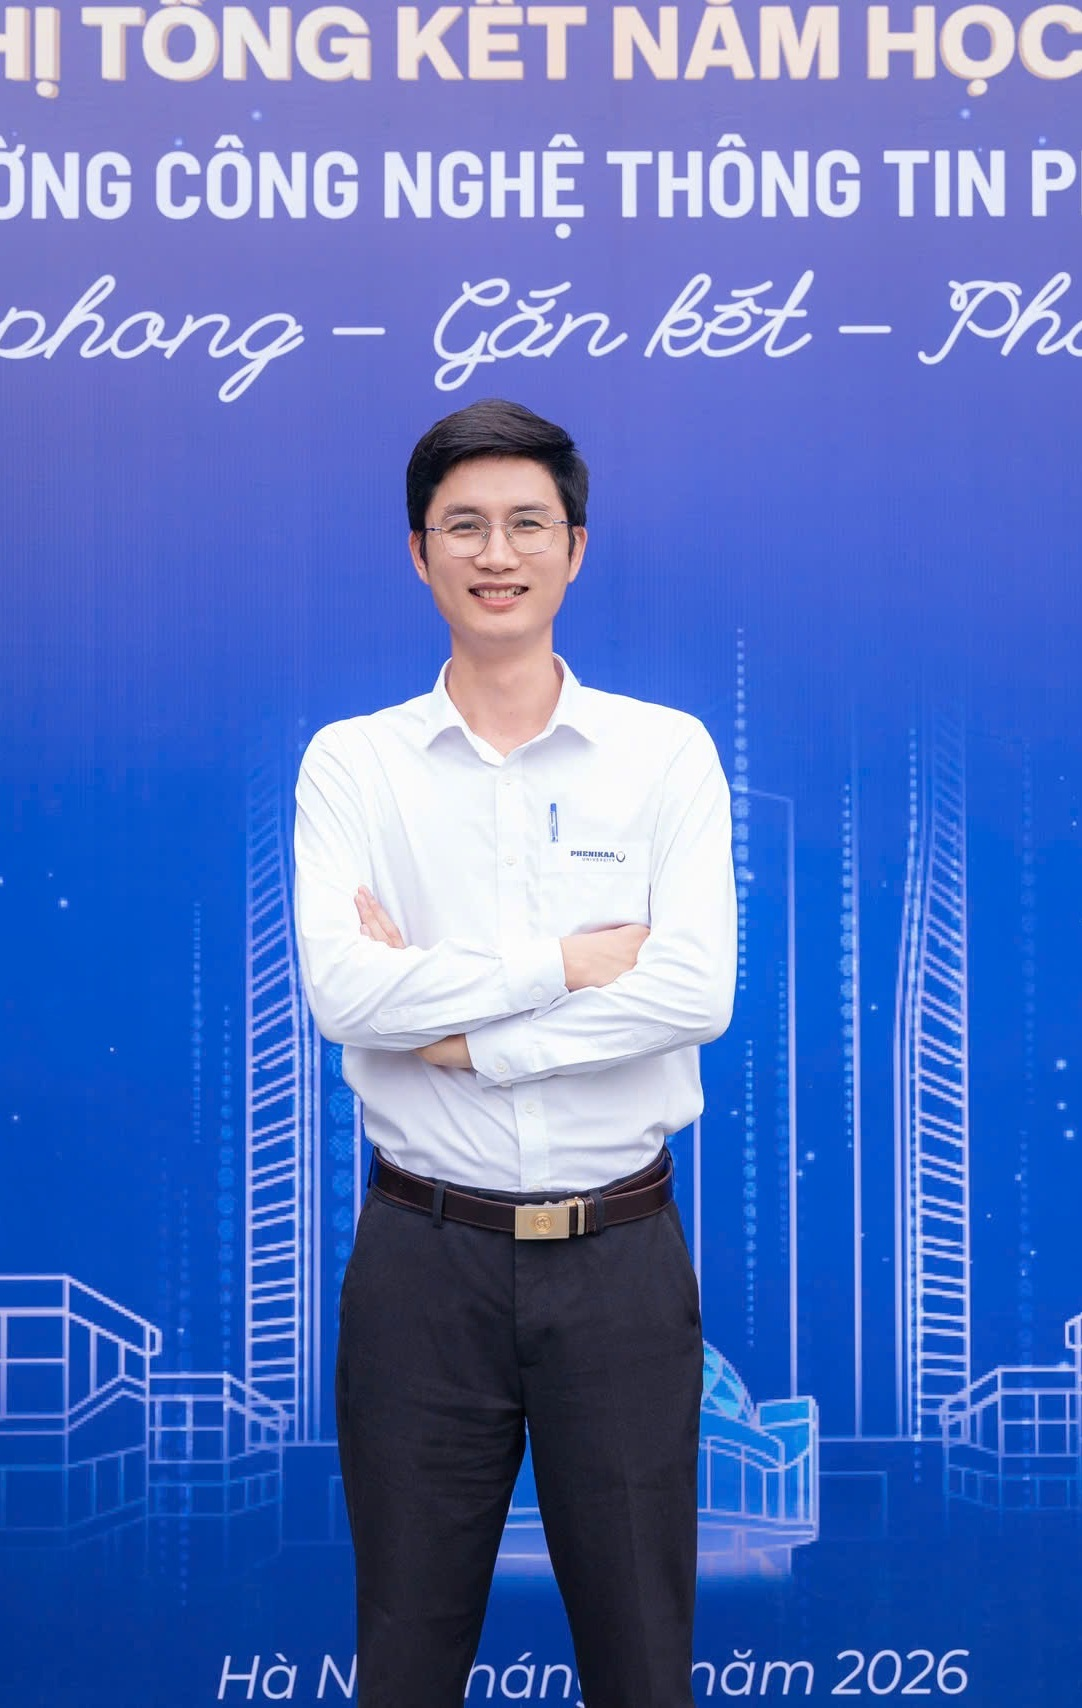
\includegraphics[width=0.34\textwidth,height=4.6cm,keepaspectratio]{Images/orlab/trandinhtan.jpg}\par
        \vspace{2pt}
        \textbf{TS. Trần Đình Tân}\\
        \textit{Cán bộ hướng dẫn}
    \end{minipage}
    \vspace{2pt}
    \caption{Lãnh đạo và cán bộ hướng dẫn khoa học tại phòng thí nghiệm ORLab.}
    \label{fig:orlab_leadership}
\end{figure}

\begin{itemize}
    \item \textbf{Trưởng phòng thí nghiệm}: PGS.TS. Phạm Văn Cảnh chịu trách nhiệm định hướng chiến lược học thuật tổng thể, chủ trì các đề tài khoa học trọng điểm và kết nối hợp tác quốc tế.
    \item \textbf{Cán bộ nghiên cứu và hướng dẫn}: TS. Trần Đình Tân trực tiếp định hướng chuyên môn, giao nhiệm vụ nghiên cứu và đồng hành cùng tôi trong suốt quá trình triển khai đề tài thực tập.
    \item \textbf{Thành viên nghiên cứu chủ chốt}: Các giảng viên và nhà nghiên cứu như TS. Dương Thị Kim Huyền, TS. Hà Thị Kim Dung, TS. Tạ Thúy Anh, cùng các nghiên cứu sinh tiến sĩ tích cực trao đổi học thuật và hỗ trợ kỹ thuật chuyên sâu.
    \item \textbf{Nhóm sinh viên nghiên cứu}: Trực tiếp hiện thực hóa giải thuật, chạy các kịch bản thực nghiệm trên máy chủ GPU và xây dựng báo cáo khoa học.
\end{itemize}

\section{Các hướng nghiên cứu chính của đơn vị}
\label{sec:cac_huong_nghien_cuu_orlab}

Theo định hướng chính thức từ cổng thông tin ORLab, hoạt động nghiên cứu của phòng thí nghiệm được tổ chức thành hai hướng nghiên cứu chính:

\begin{enumerate}[itemsep=1pt, parsep=0pt, topsep=2pt]
    \item \textbf{Hướng nghiên cứu 01: Tối ưu hóa}:
    \begin{itemize}[itemsep=1pt, parsep=0pt, topsep=1pt]
        \item \textit{Tối ưu hóa tổ hợp}: Phát triển các thuật toán chính xác và thuật toán xấp xỉ cho các bài toán tối ưu trên đồ thị và mạng lưới.
        \item \textit{Tối ưu hóa hàm submodular}: Khai thác tính chất suy giảm cận biên để giải quyết hiệu quả bài toán chọn tập con đại diện, nén dữ liệu và bài toán Facility Location với bảo đảm cận xấp xỉ lý thuyết.
        \item \textit{Định tuyến và lập lịch}: Ứng dụng giải quyết bài toán điều vận phương tiện VRP, lập lịch sản xuất công nghiệp và tối ưu chuỗi cung ứng.
        \item \textit{Tối ưu hóa ngẫu nhiên và bền vững}: Xây dựng các mô hình tối ưu có khả năng chống chịu nhiễu và biến động dữ liệu thực tế.
    \end{itemize}
    \item \textbf{Hướng nghiên cứu 02: Trí tuệ nhân tạo}:
    \begin{itemize}[itemsep=1pt, parsep=0pt, topsep=1pt]
        \item \textit{Học máy và học sâu}: Xây dựng các kiến trúc mô hình học biểu diễn dữ liệu quy mô lớn.
        \item \textit{Học tăng cường}: Ứng dụng trong việc tự động hóa quá trình ra quyết định và điều khiển thông minh.
        \item \textit{Học liên kết}: Bảo mật dữ liệu phân tán trong huấn luyện mô hình.
        \item \textit{Mô hình ngôn ngữ lớn và hệ thống đa tác tử}: Nghiên cứu cơ chế phối hợp tác tử tự trị và ứng dụng mô hình ngôn ngữ lớn vào giải quyết các bài~toán~phức~tạp.
    \end{itemize}
\end{enumerate}

\section{Sự chuẩn bị của tôi cho kỳ thực tập công nghiệp}
\label{sec:chuan_bi_thuc_tap}

Để đáp ứng các yêu cầu nghiên cứu khắt khe và hoàn thành tốt nhiệm vụ được giao tại phòng thí nghiệm ORLab, tôi đã chủ động chuẩn bị đầy đủ cả về kiến thức chuyên môn lẫn kỹ~năng~thực~hành:

\subsection{Về cơ sở thực tập}
Tôi đã chủ động tìm hiểu các công trình khoa học đã công bố của ORLab, theo dõi thông tin trên website của Lab, tham gia các buổi seminar học thuật và liên hệ trực tiếp với TS. Trần Đình Tân để được tiếp nhận vào nhóm nghiên cứu về tối ưu hóa chọn tập protein đại~diện một cách hiệu quả.

\subsection{Về kiến thức và kỹ năng kỹ thuật}
Tôi đã củng cố vững chắc các nền tảng công nghệ phục vụ trực tiếp cho đề tài nghiên cứu:
\begin{itemize}[itemsep=1pt, parsep=0pt, topsep=2pt]
    \item \textbf{Nền tảng toán học}: Ôn tập đại số tuyến tính, lý thuyết đồ thị, giải tích ma trận và lý thuyết tối ưu hóa hàm submodular có ràng buộc lực lượng.
    \item \textbf{Kỹ năng lập trình chuyên nghiệp}: Sử dụng thành thạo Python 3.12, trình quản lý môi trường hiện đại uv, cùng các thư viện khoa học lõi gồm PyTorch, Biopython, NumPy, SciPy và Scikit-learn.
    \item \textbf{Kỹ thuật tăng tốc phần cứng}: Nắm vững kỹ thuật lập trình vector hóa trên GPU CUDA nhằm tính toán song song ma trận tương đồng kích thước lớn với tốc độ và hiệu năng cao.
\end{itemize}
